\section{Documentation for programmers}
\subsection{Specification}
The aim of this program is to simulate an alarm clock. The functionality it provides is the following:
\begin{itemize}
	\item Displaying the time flowing in the following format: \texttt{hh:mm:ss};
	\item When the time reaches the value 23:59:59, it jumps to 00:00:00;
	\item When the board is powered up, the user is asked to set both the clock's time and the wake up time;
	\item The board does not ring when it wakes up. Instead, a led blinks for 30 seconds;
	\item When the clock is running it is possible to change both the clock's and the wake up time without influencing the clock.
\end{itemize}

\subsection{Structural choices}
The program operates by using interrupts. 

\textbf{BUT1} and \textbf{BUT2} are mapped to high priority interrupts, respectively \textbf{INT3} and \textbf{INT1}. The function \texttt{HighISR} handles a pressure on one of these two buttons. Since it is a bad practice to have ``fat'' interrupt handlers, the function only acts on two flags to let the \texttt{main} know what happened. These flags are the fields \texttt{button1} and \texttt{button2} of the \texttt{interrupts} struct type. The \texttt{main} then acts accordingly, by calling either \texttt{HandleButton1Pressure} or \\\texttt{HandleButton2Pressure}. Their behavior depends on the actual state of the timer. On one hand they are used to set both the clock's and the wake up time. On the other hand, they are used to begin a setting procedure. The action is determined by one of the following three flags, forming the \texttt{flags} struct type:
\begin{itemize}
	\item \texttt{time\_setting\_procedure}, high if and only if the user is setting the clock's time;
	\item \texttt{awake\_setting\_procedure}, high if and only if the user is setting the wake up time;
	\item \texttt{set}, high if and only if the initial setting procedure has been completed.
\end{itemize}

Please notice that once \texttt{flags.set} is set at 1, it never changes this value. On the other hand, both \texttt{time\_setting\_procedure} and \texttt{awake\_setting\_procedure} are reset when the corresponding setting procedure ends, and set at 1 when it restarts.

Three different struct types are used to store time values:
\begin{itemize}
	\item \texttt{clock\_time} represents the flowing time and is shown when no setting procedure is underway. It contains three fields: \texttt{hours}, \texttt{minutes} and \texttt{seconds};
	\item \texttt{awake\_time} represents the wake up time. This struct only contains \texttt{hours} and \texttt{minutes};
	\item \texttt{setting\_values} represents a time value which will be copied into \\\texttt{clock\_time} at the end of the setting procedure. We use a separate struct for this so that the current, ongoing, time value is not affected by the user. On a different version providing the possibility to cancel a setting procedure, this copy would be useful in order to preserve the ongoing value to be modified. Since the user is not allowed to set the seconds, this struct only contains two fields: \texttt{hours} and \texttt{minutes}.
\end{itemize}

We use a char array, \texttt{time\_value}, to store the time values as a string. This array is then used during the LCD display updates. The main entry point for these updates is the function \texttt{UpdateDisplay}. It accepts one parameter representing the current timer's state. This state is one of the three values of the \texttt{display\_states} enum type:
\begin{itemize}
	\item \texttt{CLOCK\_SETTING}, corresponding to the clock's time setting procedure;
	\item \texttt{TIMER\_SETTING}, corresponding to the awake time setting procedure;
	\item \texttt{TIME\_FLOWING}, corresponding to the time-only view;
\end{itemize}
When needed, we update this array using the function \texttt{ultoa} and then we display the new time. This function is helpful, because it inserts a null character (\texttt{'$\backslash$0'}) after the converted value, such that the display update does not require the entire array to be shown. For instance, when the user is setting the hours value only two digits (and consequently two characters) have to be displayed: there is no need to display the minutes value, which remains unchanged during the hours setting. 

Another possibility would be to use \texttt{sprintf} instead of \texttt{ultoa}. The former simplifies the string formatting, since it is possible to format the value with two digits (by providing \texttt{$"$\%2d$"$} as a parameter). Nonetheless, the use (and consequently the inclusion) of this function increases the space occupied by the program. We achieve the same result with an additional check on the generated string. We enforce by constructions that the values to be converted are always valid time values (range 0-59). Consequently, the generated string has always at least two characters: the number (in case it is less than 10) and the null character. By accessing the second character (which is always well defined), and comparing it with \texttt{'$\backslash$0'} we can discriminate two different cases:
\begin{enumerate}
	\item They are equal. The value comprises only one digit and we need to prepend (in \texttt{time\_value}) a $0$;
	\item They are not equal. The value comprises two digits and there is no need to further manipulate its char representation.
\end{enumerate}
The \texttt{time\_value}'s dereferentiation correctness is ensured by construction. We initialize and manipulate its elements making sure we never access an uninitialized element or an out-of-bounds location.

\subsection{System clock frequency measurement}
The clock frequency of the board that is being used (Olimex PIC-MAXI-WEB) is set at boot time by the tftp server. To know exactly at what frequency the board is running, a test routine has been performed with an ad-hoc software (\texttt{clkfreq.c}).

To take the measurement another time reference is needed; the basic idea is to count how many execution clock ticks happen in a certain period, and obtain the frequency from the inverse relationship.

In addition to the main clock, a second - low-frequency - oscillator (32.768 kHz) is present inside the Olimex board; using the full 16-bit register it is possible to count up to 2 seconds.

The \texttt{timer1} has been configured to make use of the external oscillator and generate a period of 2 seconds, while the \texttt{timer0} counts each execution clock tick on a 8 bit register; whenever the latter counter is full, an Interrupt Service Routine is called to increase a variable, which thus represents the number of overflows of the \texttt{timer0}.\\

\begin{figure}[h]
	\centering
	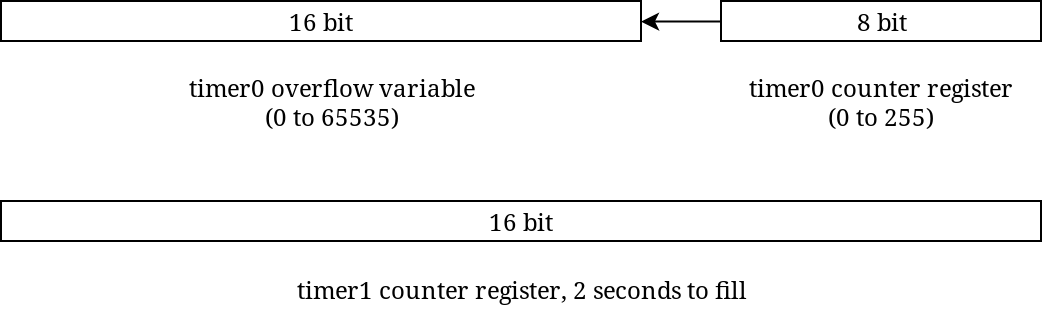
\includegraphics[width=0.7\linewidth]{images/timers}
	\label{fig:timers}
\end{figure}

\flushleft
After the predefined period (2 seconds) has passed, the value of the overflow variable is printed to the LCD screen. The clock frequency can be calculated using these formulas:

$$ f_{clk,exec} = \frac{t0\_overflows \cdot 2^8}{2}\, \left[{\frac{ticks}{seconds} = Hz}\right]$$
$$ f_{clk,sys} = 4 \cdot f_{clk,exec}\,\left[Hz\right] $$

\flushleft
The testing routine, after a (short) startup stabilization time, shows a value equal to:
$$ t0\_overflows = 48825 $$
Which leads to $f_{clk,exec} = 6.2496\,MHz$ and $f_{clk,sys} = 24.9984\,Mhz \approx 25\,Mhz$.\\
\flushleft
A couple of final considerations on this method:
\begin{itemize}
	\item With the current registers configuration, the system clock measurement range is from $512\,Hz$ to $33.55\,MHz$. Precedent experiments had been performed to make sure that the clock frequency was inside this range (it can be set up to $41.667\,MHz$ on the Olimex board).
	\item Being the number of overflows very high, the measurement uncertainty is quite low; even assuming an uncertainty equal to 50 overflows (12800 ticks!) the relative error is around 0.1\%.
\end{itemize}